% !TEX encoding = UTF-8
% !TEX TS-program = pdflatex
% !TEX root = tesi.tex
% !TEX spellcheck = it-IT

% PDF/A filecontents
\RequirePackage{filecontents}
\begin{filecontents*}{\jobname.xmpdata}
  \Title{Valutazione sperimentale di Hotmoka Blockchain}
  \Author{Filippo Fantinato}
  \Language{it-IT}
  \Subject{Tesi di laurea triennale}
  \Keywords{Blockchain\sep NFT\sep Hotmoka\sep Ethereum\sep Smart contract}
\end{filecontents*}

\documentclass[10pt,                    % corpo del font principale
               a4paper,                 % carta A4
               twoside,                 % impagina per fronte-retro
               openright,               % inizio capitoli a destra
               english,                 
               italian,                 
               ]{book}

%**************************************************************
% Importazione package
%************************************************************** 

\PassOptionsToPackage{dvipsnames}{xcolor} % colori PDF/A

\usepackage{colorprofiles}

\usepackage[a-2b,mathxmp]{pdfx}[2018/12/22]
                                        % configurazione PDF/A
                                        % validare in https://www.pdf-online.com/osa/validate.aspx

%\usepackage{amsmath,amssymb,amsthm}    % matematica

\usepackage[T1]{fontenc}                % codifica dei font:
                                        % NOTA BENE! richiede una distribuzione *completa* di LaTeX

\usepackage[utf8]{inputenc}             % codifica di input; anche [latin1] va bene
                                        % NOTA BENE! va accordata con le preferenze dell'editor

\usepackage[english, italian]{babel}    % per scrivere in italiano e in inglese;
                                        % l'ultima lingua (l'italiano) risulta predefinita

\usepackage{bookmark}                   % segnalibri

\usepackage{caption}                    % didascalie

\usepackage{chngpage,calc}              % centra il frontespizio

\usepackage{csquotes}                   % gestisce automaticamente i caratteri (")

\usepackage{emptypage}                  % pagine vuote senza testatina e piede di pagina

\usepackage{epigraph}			% per epigrafi

\usepackage{eurosym}                    % simbolo dell'euro

%\usepackage{indentfirst}               % rientra il primo paragrafo di ogni sezione

\usepackage{graphicx}                   % immagini

\usepackage{hyperref}                   % collegamenti ipertestuali

\usepackage[binding=5mm]{layaureo}      % margini ottimizzati per l'A4; rilegatura di 5 mm

\usepackage{listings}                   % codici

\usepackage{microtype}                  % microtipografia

\usepackage{mparhack,fixltx2e,relsize}  % finezze tipografiche

\usepackage{nameref}                    % visualizza nome dei riferimenti                                      
\usepackage[font=small]{quoting}        % citazioni

\usepackage{subfig}                     % sottofigure, sottotabelle

\usepackage[italian]{varioref}          % riferimenti completi della pagina

\usepackage{booktabs}                   % tabelle                                       
\usepackage{tabularx}                   % tabelle di larghezza prefissata   
\usepackage{multirow}
\usepackage{longtable}                  % tabelle su più pagine       
\usepackage{tabu}                                 
\usepackage{ltxtable}                   % tabelle su più pagine e adattabili in larghezza

\usepackage[toc, acronym]{glossaries}   % glossario
                                        % per includerlo nel documento bisogna:
                                        % 1. compilare una prima volta tesi.tex;
                                        % 2. eseguire: makeindex -s tesi.ist -t tesi.glg -o tesi.gls tesi.glo
                                        % 3. eseguire: makeindex -s tesi.ist -t tesi.alg -o tesi.acr tesi.acn
                                        % 4. compilare due volte tesi.tex.

\usepackage[backend=biber,style=verbose-ibid,hyperref,backref]{biblatex}
                                        % eccellente pacchetto per la bibliografia; 
                                        % produce uno stile di citazione autore-anno; 
                                        % lo stile "numeric-comp" produce riferimenti numerici
                                        % per includerlo nel documento bisogna:
                                        % 1. compilare una prima volta tesi.tex;
                                        % 2. eseguire: biber tesi
                                        % 3. compilare ancora tesi.tex.

%**************************************************************
% file contenente le impostazioni della tesi
%**************************************************************

%**************************************************************
% Frontespizio
%**************************************************************

% Autore
\newcommand{\myName}{Filippo Fantinato}                                    
\newcommand{\myTitle}{Valutazione sperimentale di Hotmoka Blockchain}

% Tipo di tesi                   
\newcommand{\myDegree}{Tesi di laurea}

% Università             
\newcommand{\myUni}{Università degli Studi di Padova}

% Facoltà       
\newcommand{\myFaculty}{Corso di Laurea in Informatica}

% Dipartimento
\newcommand{\myDepartment}{Dipartimento di Matematica "Tullio Levi-Civita"}

% Titolo del relatore
\newcommand{\profTitle}{Prof.}

% Relatore
\newcommand{\myProf}{Tullio Vardanega}

% Luogo
\newcommand{\myLocation}{Padova}

% Anno accademico
\newcommand{\myAA}{2020-2021}

% Data discussione
\newcommand{\myTime}{Luglio 2021}


%**************************************************************
% Impostazioni di impaginazione
% see: http://wwwcdf.pd.infn.it/AppuntiLinux/a2547.htm
%**************************************************************

\setlength{\parindent}{14pt}   % larghezza rientro della prima riga
\setlength{\parskip}{0pt}   % distanza tra i paragrafi


%**************************************************************
% Impostazioni di biblatex
%**************************************************************
\bibliography{bibliografia} % database di biblatex 

\defbibheading{bibliography} {
    \cleardoublepage
    \phantomsection 
    \addcontentsline{toc}{chapter}{\bibname}
    \chapter*{\bibname\markboth{\bibname}{\bibname}}
}

\setlength\bibitemsep{1.5\itemsep} % spazio tra entry

\DeclareBibliographyCategory{opere}
\DeclareBibliographyCategory{web}

\addtocategory{opere}{womak:lean-thinking}
\addtocategory{web}{site:agile-manifesto}

\defbibheading{opere}{\section*{Riferimenti bibliografici}}
\defbibheading{web}{\section*{Siti Web consultati}}


%**************************************************************
% Impostazioni di caption
%**************************************************************
\captionsetup{
    tableposition=top,
    figureposition=bottom,
    font=small,
    format=hang,
    labelfont=bf
}

%**************************************************************
% Impostazioni di glossaries
%**************************************************************

%**************************************************************
% Acronimi
%**************************************************************
\renewcommand{\acronymname}{Acronimi e abbreviazioni}

\newacronym[description={\glslink{ICT}{Information and Communications Technology}}]
    {ict}{ICT}{Information and Communications Technology}

\newacronym[description={\glslink{apig}{Application Program Interface}}]
    {api}{API}{Application Program Interface}

\newacronym[description={\glslink{umlg}{Unified Modeling Language}}]
    {uml}{UML}{Unified Modeling Language}

%**************************************************************
% Glossario
%**************************************************************
\renewcommand{\glossaryname}{Glossario}
% \renewcommand{\glossar}{Glossario}

\newglossaryentry{ICT}{
    name=\glslink{ict}{ICT},
    text=Information and Communications Technology,
    description={Con il termine \textit{Information and Communications Technology}, si intende l'uso della tecnologia nella gestione e nel trattamento delle informazioni. Include tutti gli ambiti professionali che riguardano la progettazione e lo sviluppo tecnico della comunicazione digitale}
}

\newglossaryentry{System Integrator}
{
    name=System Integrator,
    description={Con il termine inglese \textit{System Integrator} viene indicata un'azienda che si occupa dell'integrazione di sistemi. Il suo compito è quello di far dialogare impianti diversi tra di loro, allo scopo di creare una nuova struttura funzionale che possa utilizzare sinergicamente le potenzialità degli impianti d'origine e creando quindi funzionalità originariamente non presenti}
}

\newglossaryentry{on premises}{
    name={On premises},
    text={on premises},
    description={In informatica con il termine \textit{on premises} si indica l'installazione del \textit{software} direttamente sulla macchina locale}
}

\newglossaryentry{Single Page Application}{
    name=Single Page Application,
    text=Single Page Application,
    description={Per \textit{Single Page Application} si intende qualsiasi applicazione web che interagisce con l'utente aggiornando le parti della pagina con dati prelevati direttamente dal server}
}

\newglossaryentry{Single File Components}{
    name=Single File Components,
    text=Single File Components,
    description={È la principale caratteristica del \textit{framework} Vue.js e permette di definire il codice di \textit{markup}, la logica e lo stile direttamente all'interno dello stesso file}
}
 % database di termini
\makeglossaries


%**************************************************************
% Impostazioni di graphicx
%**************************************************************
\graphicspath{{immagini/}} % cartella dove sono riposte le immagini


%**************************************************************
% Impostazioni di hyperref
%**************************************************************
\hypersetup{
    %hyperfootnotes=false,
    %pdfpagelabels,
    %draft,	% = elimina tutti i link (utile per stampe in bianco e nero)
    colorlinks=true,
    linktocpage=true,
    pdfstartpage=1,
    pdfstartview=,
    % decommenta la riga seguente per avere link in nero (per esempio per la stampa in bianco e nero)
    %colorlinks=false, linktocpage=false, pdfborder={0 0 0}, pdfstartpage=1, pdfstartview=FitV,
    breaklinks=true,
    pdfpagemode=UseNone,
    pageanchor=true,
    pdfpagemode=UseOutlines,
    plainpages=false,
    bookmarksnumbered,
    bookmarksopen=true,
    bookmarksopenlevel=1,
    hypertexnames=true,
    pdfhighlight=/O,
    %nesting=true,
    %frenchlinks,
    urlcolor=webbrown,
    linkcolor=RoyalBlue,
    citecolor=webgreen,
    %pagecolor=RoyalBlue,
    %urlcolor=Black, linkcolor=Black, citecolor=Black, %pagecolor=Black,
    pdftitle={\myTitle},
    pdfauthor={\textcopyright\ \myName, \myUni, \myFaculty},
    pdfsubject={},
    pdfkeywords={},
    pdfcreator={pdfLaTeX},
    pdfproducer={LaTeX}
}

%**************************************************************
% Impostazioni di itemize
%**************************************************************
% \renewcommand{\labelitemi}{$\ast$}

\renewcommand{\labelitemi}{$\bullet$}
%\renewcommand{\labelitemii}{$\cdot$}
%\renewcommand{\labelitemiii}{$\diamond$}
%\renewcommand{\labelitemiv}{$\ast$}


%**************************************************************
% Impostazioni di listings
%**************************************************************
\lstset{
    language=[LaTeX]Tex,%C++,
    keywordstyle=\color{RoyalBlue}, %\bfseries,
    basicstyle=\small\ttfamily,
    %identifierstyle=\color{NavyBlue},
    commentstyle=\color{Green}\ttfamily,
    stringstyle=\rmfamily,
    numbers=none, %left,%
    numberstyle=\scriptsize, %\tiny
    stepnumber=5,
    numbersep=8pt,
    showstringspaces=false,
    breaklines=true,
    frameround=ftff,
    frame=single
} 


%**************************************************************
% Impostazioni di xcolor
%**************************************************************
\definecolor{webgreen}{rgb}{0,.5,0}
\definecolor{webbrown}{rgb}{.6,0,0}


%**************************************************************
% Altro
%**************************************************************

\newcommand{\omissis}{[\dots\negthinspace]} % produce [...]

% eccezioni all'algoritmo di sillabazione
\hyphenation
{
    ma-cro-istru-zio-ne
    gi-ral-din
}

\newcommand{\sectionname}{sezione}
\addto\captionsitalian{\renewcommand{\figurename}{Figura}
                       \renewcommand{\tablename}{Tabella}}

\newcommand{\glsfirstoccur}{\ap{{[g]}}}

\newcommand{\intro}[1]{\textit{\textsf{#1}}}

%**************************************************************
% Environment per ``rischi''
%**************************************************************
\newcounter{riskcounter}                % define a counter
\setcounter{riskcounter}{0}             % set the counter to some initial value

%%%% Parameters
% #1: Title
\newenvironment{risk}[1]{
    \refstepcounter{riskcounter}        % increment counter
    \par \noindent                      % start new paragraph
    \textbf{\arabic{riskcounter}. #1}   % display the title before the 
                                        % content of the environment is displayed 
}{
    \par\medskip
}

\newcommand{\riskname}{Rischio}

\newcommand{\riskdescription}[1]{\textbf{\\Descrizione:} #1.}

\newcommand{\risksolution}[1]{\textbf{\\Soluzione:} #1.}

\renewcommand{\arraystretch}{1.2}

%**************************************************************
% Environment per ``use case''
%**************************************************************
\newcounter{usecasecounter}             % define a counter
\setcounter{usecasecounter}{0}          % set the counter to some initial value

%%%% Parameters
% #1: ID
% #2: Nome
\newenvironment{usecase}[2]{
    \renewcommand{\theusecasecounter}{\usecasename #1}  % this is where the display of 
                                                        % the counter is overwritten/modified
    \refstepcounter{usecasecounter}             % increment counter
    \vspace{10pt}
    \par \noindent                              % start new paragraph
    {\large \textbf{\usecasename #1: #2}}       % display the title before the 
                                                % content of the environment is displayed 
    \medskip
}{
    \medskip
}

\newcommand{\usecasename}{UC}

\newcommand{\usecaseactors}[1]{\textbf{\\Attori Principali:} #1. \vspace{4pt}}
\newcommand{\usecasepre}[1]{\textbf{\\Precondizioni:} #1. \vspace{4pt}}
\newcommand{\usecasedesc}[1]{\textbf{\\Descrizione:} #1. \vspace{4pt}}
\newcommand{\usecasepost}[1]{\textbf{\\Postcondizioni:} #1. \vspace{4pt}}
\newcommand{\usecasealt}[1]{\textbf{\\Scenario Alternativo:} #1. \vspace{4pt}}

%**************************************************************
% Environment per ``namespace description''
%**************************************************************

\newenvironment{namespacedesc}{
    \vspace{10pt}
    \par \noindent                              % start new paragraph
    \begin{description} 
}{
    \end{description}
    \medskip
}

\newcommand{\classdesc}[2]{\item[\textbf{#1:}] #2}
                     % file con le impostazioni personali

\begin{document}
%**************************************************************
% Materiale iniziale
%**************************************************************
\frontmatter
% !TEX encoding = UTF-8
% !TEX TS-program = pdflatex
% !TEX root = ../tesi.tex

%**************************************************************
% Frontespizio 
%**************************************************************
\begin{titlepage}

\begin{center}

\begin{LARGE}
\textbf{\myUni}\\
\end{LARGE}

\vspace{10pt}

\begin{Large}
\textsc{\myDepartment}\\
\end{Large}

\vspace{10pt}

\begin{large}
\textsc{\myFaculty}\\
\end{large}

\vspace{30pt}
\begin{figure}[htbp]
\begin{center}

\includegraphics[height=6cm]{logo-unipd}
\end{center}
\end{figure}
\vspace{30pt} 

\begin{LARGE}
\begin{center}
\textbf{\myTitle}\\
\end{center}
\end{LARGE}

\vspace{10pt} 

\begin{large}
\textsl{\myDegree}\\
\end{large}

\vspace{40pt} 

\begin{large}
\begin{flushleft}
\textit{Relatore}\\ 
\vspace{5pt} 
\profTitle{} \myProf
\end{flushleft}

\vspace{0pt} 

\begin{flushright}
\textit{Laureando}\\ 
\vspace{5pt} 
\myName
\end{flushright}
\end{large}

\vspace{40pt}

\line(1, 0){338} \\
\begin{normalsize}
\textsc{Anno Accademico \myAA}
\end{normalsize}

\end{center}
\end{titlepage} 
% !TEX encoding = UTF-8
% !TEX TS-program = pdflatex
% !TEX root = ../tesi.tex

%**************************************************************
% Colophon
%**************************************************************
\clearpage
\phantomsection
\thispagestyle{empty}

\hfill

\vfill

\noindent\myName: \textit{\myTitle,}
\myDegree,
\textcopyright\ \myTime.
% % !TEX encoding = UTF-8
% !TEX TS-program = pdflatex
% !TEX root = ../tesi.tex

%**************************************************************
% Dedica
%**************************************************************
\cleardoublepage
\phantomsection
\thispagestyle{empty}
% \pdfbookmark{Dedica}{Dedica}

\vspace*{3cm}

\begin{center}
"You can never understand everything. 
But, you should push yourself to understand the system." \\ \medskip
--- Ryan Dahl 
\end{center}

% !TEX encoding = UTF-8
% !TEX TS-program = pdflatex
% !TEX root = ../tesi.tex

%**************************************************************
% Sommario
%**************************************************************
\cleardoublepage
\phantomsection
\pdfbookmark{Sommario}{Sommario}
\begingroup
\let\clearpage\relax
\let\cleardoublepage\relax
\let\cleardoublepage\relax

\chapter*{Sommario}

Il presente documento descrive il tirocinio da me svolto presso l'azienda Sync Lab s.r.l durante il periodo che va dal 03-05-2021 al 25-06-2021.
L'esperienza di tirocinio ha avuto una durata complessiva di 320 ore ed è stata supervisionata e coordinata sia dal mio tutor aziendale, l'ingegnere Fabio Pallaro, sia dal mio relatore presso l'ateneo, \profTitle{} \myProf. \\

\noindent Lo scopo dello stage era di realizzare uno \textit{smart contract} che gestisse la compravendita di NFT. Questo \textit{smart contract} doveva essere implementato attraverso gli standard NFT delle \textit{blockchain} Ethereum e HotMoka. Inoltre ne è seguito anche lo sviluppo di una libreria che ha permesso alla piattaforma NFTLab di comunicare con la blockchain.

\noindent Il percorso di tirocinio ha richiesto lo studio della tecnologia \textit{blockchain}, approfondendo Ethereum e HotMoka, e l'implementazione di \textit{smart contract} attraverso i linguaggi di programmazione Solidity e Takamaka seguendo lo standard ERC721. \\

\noindent Ho suddiviso il presente documento in 4 capitoli e 3 sezioni di supporto:
\begin{itemize}
  \item \hyperref[cap:contesto-aziendale]{\textbf{Capitolo 1}}: presentazione del contesto organizzativo e produttivo aziendale, con approfondimento sui processi aziendali interni e sulla propensione all' innovazione;

  \item \hyperref[cap:stage]{\textbf{Capitolo 2}}: presentazione dell'offerta di stage con gli obiettivi, i vincoli e le motivazioni che mi hanno spinto a scegliere l'azienda Sync Lab; 
  
  \item \hyperref[cap:nftlab]{\textbf{Capitolo 3}}: presentazione dettagliata del progetto con le relative fasi, introduzione delle tecnologie trattate e delle soluzioni progettuali attuate per la realizzazione dei prodotti attesi dall'azienda;
  
  \item \hyperref[cap:valutazione-finale]{\textbf{Capitolo 4}}: valutazione retrospettiva del percorso di tirocinio, riguardante gli obiettivi raggiunti, le difficoltà e le competenze professionali maturate;
  
  \item \textbf{Glossario}: al suo interno sono stati riportati tutti i termini ambigui;
  
  \item \textbf{Acronimi}: al suo interno sono stati riportati tutti gli acronimi;

  \item \hyperref[cap:bibliografia-sitografia]{\textbf{Bibliografia e Sitografia}}: al suo interno sono stati riportati tutti i libri e siti dai quali ho reperito le informazioni.
\end{itemize}

%\vfill
%
%\selectlanguage{english}
%\pdfbookmark{Abstract}{Abstract}
%\chapter*{Abstract}
%
%\selectlanguage{italian}

\endgroup

\vfill


% % !TEX encoding = UTF-8
% !TEX TS-program = pdflatex
% !TEX root = ../tesi.tex

%**************************************************************
% Ringraziamenti
%**************************************************************
\cleardoublepage
\phantomsection
\pdfbookmark{Ringraziamenti}{ringraziamenti}

\begin{flushright}{
	\slshape    
	``You can never understand everything. 
	
	But, you should push yourself to understand the system.''} \\ 
	\medskip
    --- Ryan Dahl
\end{flushright}


\bigskip

\begingroup
\let\clearpage\relax
\let\cleardoublepage\relax
\let\cleardoublepage\relax

\chapter*{Ringraziamenti}

\noindent \textit{Desidero innanzitutto ringragiare il Prof. \myProf, relatore della mia tesi, per avermi seguito durante il percorso di stage e per il preciso aiuto che mi ha fornito durante la stesura della tesi.} \\

\noindent \textit{Grazie in particolare al mio tutor aziendale, l'ingegnere Fabio Pallaro, per accettato nella sua azienda e per avermi coinvolto nel progetto a cui ho collaborat, il quale è stato molto utile per la mia formazione e crescita personale.}

\noindent \textit{Un grazie di cuore va a tutta la mia famiglia, in particolare ai miei genitori Alessandra Galassi e Roberto Fantinato, per avermi supportato. Ringrazio la mia fidanzata Alice Gasparini per il sostegno e la pazienza nei miei confronti.}\\

\noindent \textit{Infine ringrazio tutte le persone che ho conosciuto durante questo percorso e i miei amici che mi sono stati a fianco durante questi anni di studio.}\\
\bigskip

\noindent\textit{\myLocation, \myTime}
\hfill \myName

\endgroup


% !TEX encoding = UTF-8
% !TEX TS-program = pdflatex
% !TEX root = ../tesi.tex

%**************************************************************
% Indici
%**************************************************************
\cleardoublepage
\pdfbookmark{\contentsname}{tableofcontents}
\setcounter{tocdepth}{2}
\tableofcontents
%\markboth{\contentsname}{\contentsname} 
\clearpage

\begingroup 
    \let\clearpage\relax
    \let\cleardoublepage\relax
    \let\cleardoublepage\relax
    %*******************************************************
    % Elenco delle figure
    %*******************************************************    
    \phantomsection
    \pdfbookmark{\listfigurename}{lof}
    \listoffigures

    \vspace*{8ex}

    %*******************************************************
    % Elenco delle tabelle
    %*******************************************************
    \phantomsection
    \pdfbookmark{\listtablename}{lot}
    \listoftables
        
    \vspace*{8ex}
\endgroup

\cleardoublepage

\cleardoublepage

%**************************************************************
% Materiale principale
%**************************************************************
\mainmatter
% \input{capitoli/introduzione}             % Introduzione
% !TEX encoding = UTF-8
% !TEX TS-program = pdflatex
% !TEX root = ../tesi.tex

\chapter{Analisi del contesto aziendale}
\label{cap:contesto-aziendale}

\section{L'azienda Sync Lab}
Sync Lab nasce come \textit{software house} nel 2002, per poi crescere rapidamente nel mercato del \gls{ICT}. In seguito ad una maturazione delle competenze tecnologiche, metodologiche ed applicative nel dominio del \textit{software}, si è tramutata in \gls{System Integrator} conquistando significative fette di mercato nei settori: \textit{mobile}, videosorveglianza e sicurezza delle infrastrutture informatiche aziendali. Attualmente vanta più di 150 clienti diretti e finali, 200 dipendenti e 5 sedi distribuite in tutta Italia. 

\begin{figure}[!h]
  \centering
  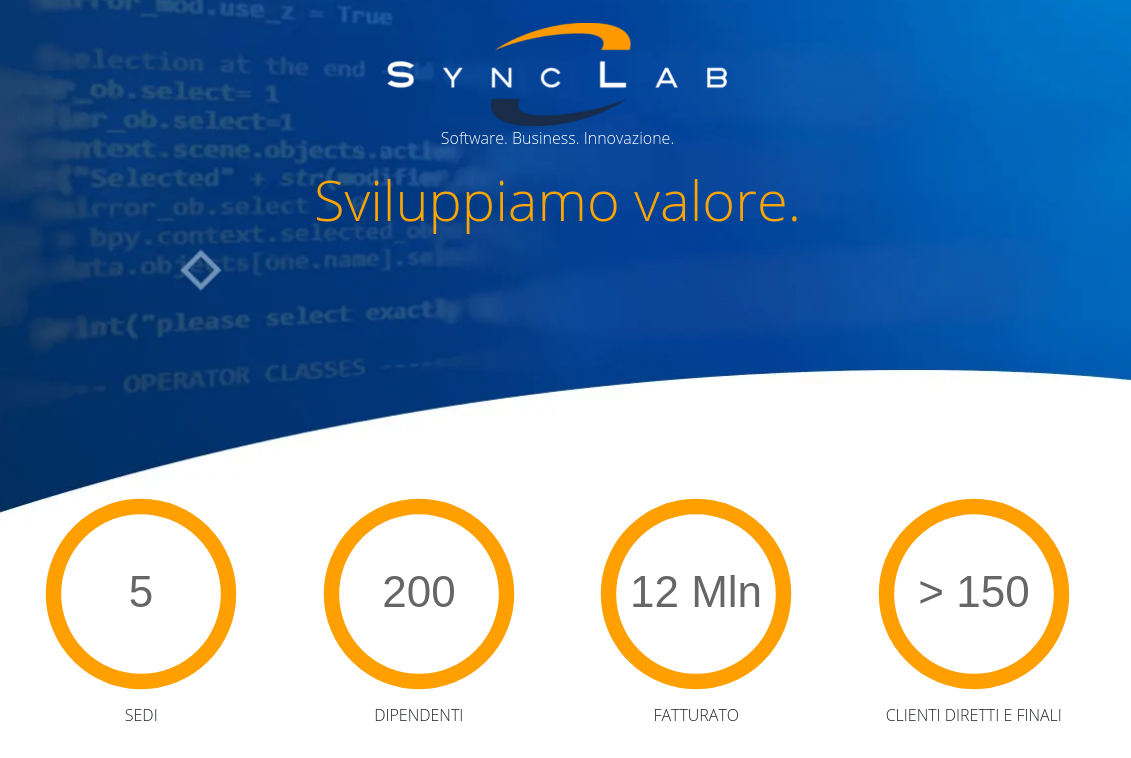
\includegraphics[width=\textwidth]{capitolo1/motto-synclab.png}
  \caption{Motto di Sync Lab e le sue statistiche}
  \textbf{Fonte}: \href{https://www.synclab.it}{https://www.synclab.it}
\end{figure}

Sync Lab consegue l'obiettivo principale di supportate il cliente nella realizzazione, messa in opera e controllo di soluzioni IT, sia dal punto di vista tecnologico, sia nel governo del cambiamento organizzativo. Nel corso degli anni ha aumentato la propria qualità organizzativa e produttiva, riuscendo ad acquisire le seguenti 4 certificazioni: ISO 9001, ISO 14001, ISO 27001 e ISO 45001.

\section{Prodotti}
Sync Lab è un'azienda di consulenza tecnologica che mette a disposizione ai suoi clienti competenze altamente qualificate ed esperienza nel dominio tecnologico. Grazie a questo, le aziende possono affrontare i cambiamenti tecnologici e di mercato rimanendo sempre competitive nell'attuale contesto di trasformazione digitale. L'azienda opera principalmente nel settore informatico e, più precisamente, nel \textit{business consultancy}, \textit{IT consultancy} e \textit{project financing}.

\begin{figure}[!h]
  \centering
  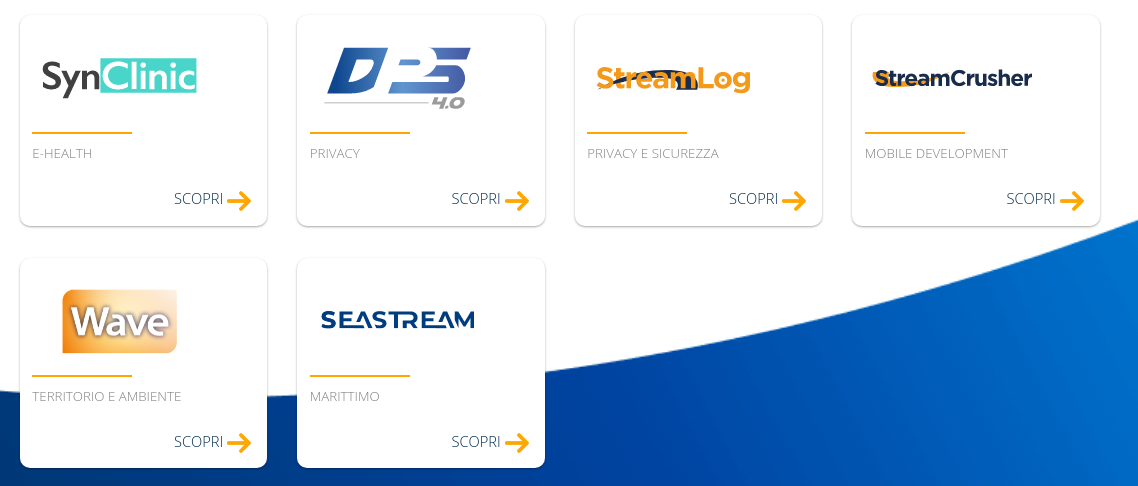
\includegraphics[width=\textwidth]{capitolo1/prodotti-synclab.png}
  \caption{I prodotti di Sync Lab}
  \textbf{Fonte}: \href{https://www.synclab.it/prodotti.php}{https://www.synclab.it/prodotti.php}
\end{figure}

\noindent In questo ambito, Sync Lab, vanta numerosi prodotti:
\begin{itemize}
  \item \textbf{SynClinic}: \textit{software} che facilita la gestione di una struttura sanitaria. Utilizzabile in \textit{cloud} e \gls{on premises}, gestisce, organizza e monitora tutte le fasi del percorso di cura del paziente, integrandosi perfettamente con i servizi regionali: fascicolo sanitario elettronico, ricetta dematerializzata e CUP regionale;
  
  \item \textbf{DPS 4.0}: consiste in una soluzione web per la gestione del GDPR, con una piattaforma guidata per aggiornare e modificare automaticamente i documenti di privacy in modo conforme agli standard di riferimento europei;
  
  \item \textbf{StreamLog}: rappresenta un sistema finalizzato al soddisfacimento dei requisiti fissati al garante, ovvero effettua il controllo degli accessi ai sistemi in modo semplice e veloce. La piattaforma è basata su \textit{framework open source} allo stato dell'arte e, in particolare, su un'innovativa tecnologia di \textit{streaming}, frutto del laboratorio di ricerca e sviluppo Sync Lab;
  
  \item \textbf{StreamCrusher}: soluzione \textit{software} che è in grado di raccogliere, indicizzare, ed interpretare la grande mole di dati che giornalmente genera qualsiasi azienda. In seguito, produrrà un resoconto con tutte le informazioni utili al centro informatico, per identificare criticità o eventuali opportunità di \textit{business};
  
  \item \textbf{Wave}: nato dal laboratorio di ricerca e sviluppo, è un \textit{plugin} della piattaforma \textit{Milestone System A/S} che permette di avere una visione geografica della distribuzione delle telecamere installate nel territorio e di capire la copertura garantita da un'installazione reale;
  
  \item \textbf{SeaStream}: piattaforma che migliora l'efficienza, la sicurezza e il processo di innovazione del settore marittimo, mettendo a disposizione strumenti per il monitoraggio e tracciamento delle navi e per la gestione portuale.  
\end{itemize}

\section{Tipologia di clientela}
La clientela che si affida a Sync Lab è molto vasta, comprendendo al suo interno aziende pubbliche e private, piccole e grandi imprese. Tutte le aziende elencate in precedenza si mettono in contatto con Sync Lab per migliorare i propri processi interni, andando così ad incrementare la propria efficienza sotto l'aspetto lavorativo. Riuscendo a soddisfare qualsiasi richiesta, Sync Lab può vantare clienti come: la regione Lazio, Trenitalia, il ministero dell'economia e delle finanze, Rai, Unicredit, Vodafone e Intesa San Paolo. Per ogni settore, l'azienda è in continua ricerca di nuove opportunità e soluzioni cercando di allargare sempre più il proprio campo applicativo per portare verso di sè una clientela più varia.

\section{Processi aziendali}
Sync Lab conta di raggiungere i propri obiettivi aziendali attraverso i processi spiegati di seguito.

\subsection{Consulenza}

\begin{figure}[!h]
  \centering
  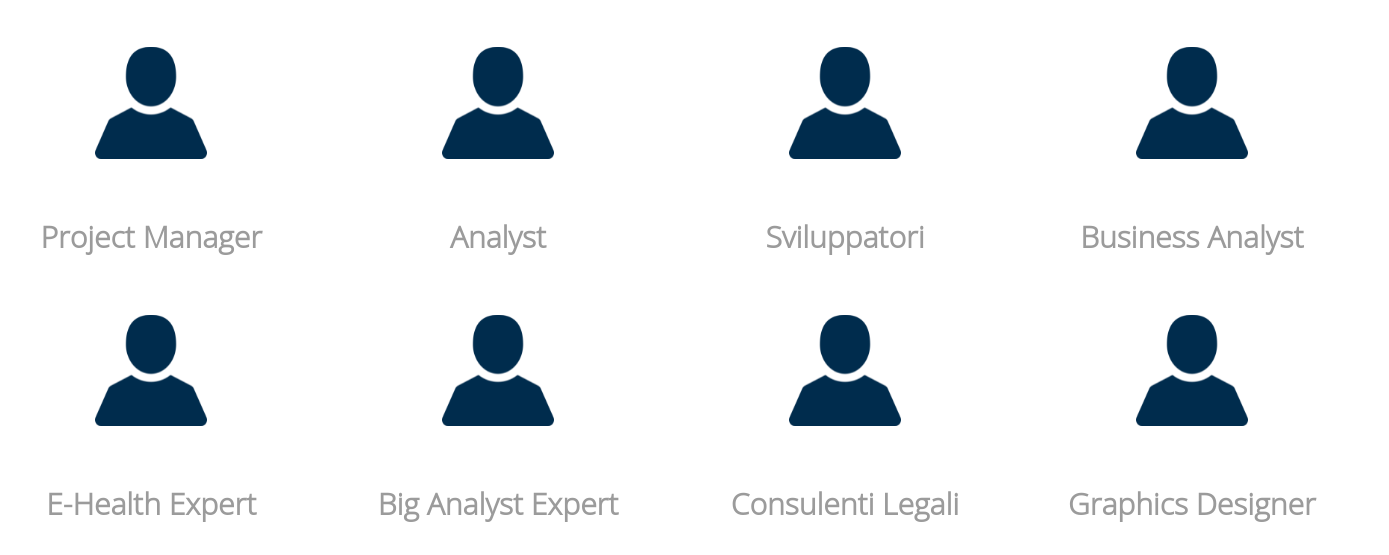
\includegraphics[width=\textwidth]{capitolo1/profili-professionali.png}
  \caption{I profili professionali messi a disposizione da Sync Lab}
  \textbf{Fonte}: \href{https://www.synclab.it/servizi-professionali.php}{https://www.synclab.it/servizi-professionali.php}
\end{figure}

In quanto \textit{partner} di grandi imprese italiane, come elencato nella sezione precedente, uno degli obiettivi principali di Sync Lab è quello di fornire una consulenza ai suoi clienti che porti un'evoluzione in termini di competitività, sviluppo e innovazione tecnologica. Inoltre, mette a disposizione un team di grande esperienza che interviene nella progettazione e realizzazione delle strategie necessari alla realizzazione di grandi progetti.

\subsection{Fornitura}
La procedura di fornitura viene avviata ogni qual volta che un cliente incarica Sync Lab per la realizzazione di un prodotto. Parallelamente, mette in atto le seguenti attività con lo scopo di migliorare questo processo:
\begin{itemize}
  \item \textbf{Miglioramento delle performance}: verifica e correzione, se necessario, delle procedure aziendali utilizzando le giuste metodologie (\textit{best practices});
  \item \textbf{Ottimizzazione della qualità}: utilizzo di \textit{design patterns} adatti al contesto aziendale;
  \item \textbf{Sviluppo delle quote di mercato}: analisi e miglioramento degli standard di qualità presso l'azienda.
\end{itemize} 

\subsection{Sviluppo}
Sync Lab fa ampio uso del modello di sviluppo Agile, più in particolare della metodologia Scrum, per permettere agli \textit{stakeholders} di seguire l'evoluzione dello sviluppo del prodotto richiesto, raccogliendo tutti i \textit{feedback} che possono essere determinanti per la loro soddisfazione. 

\paragraph{La metodologia Scrum}
Scrum è la metodologia Agile più diffusa tra i team di sviluppo. In questa metodologia gli \textit{stakeholders} hanno un ruolo fondamentale e la loro soddisfazione è determinante per la buona riuscita del progetto. Per rispondere al meglio a questa esigenza, si basa su tre pilastri fondamentali:
\begin{enumerate}
  \item \textbf{Trasparenza}: tutti coloro che partecipano ad un progetto sanno qual è lo scopo (trasparenza verticale) e sanno che cosa fanno gli altri (trasparenza orizzontale). In più, anche lo stato del progetto, con le relative statistiche, è visibile a tutti a prescindere dal livello organizzativo;
  \item \textbf{Ispezione}: ogni iterazione ed incremento vengono verificati in base alle metriche di misurazione decise, in modo tale da modificare le iterazioni successive e rendere così estremamente adattabile l'andamento del processo;
  \item \textbf{Adattamento}: è la conseguenza dell'ispezione e significa che al posto di seguire un piano preordinato, il team di sviluppo pianifica in base ai risultati dell'ispezione per apportare il maggior valore al cliente finale.
\end{enumerate}

\clearpage

\begin{figure}[h!]
  \centering
  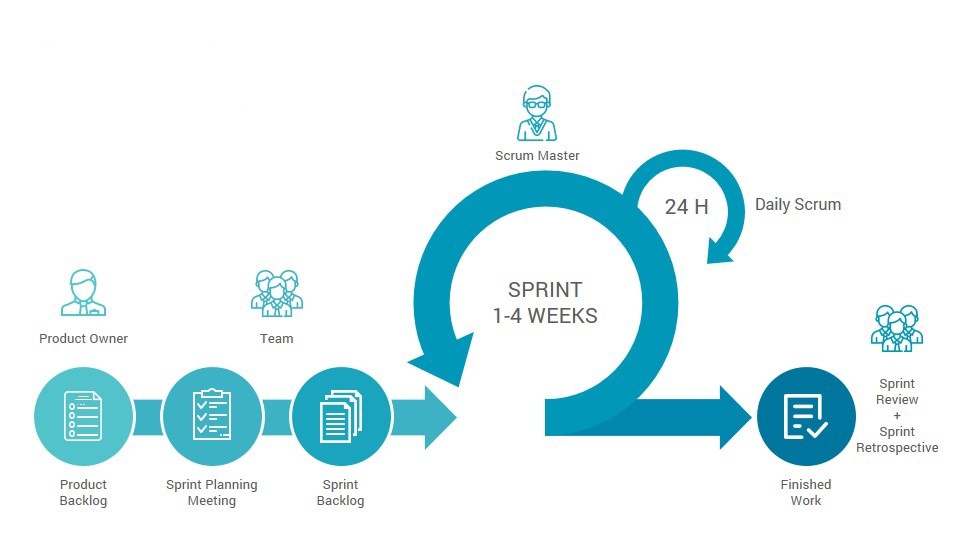
\includegraphics[width=0.8\textwidth]{capitolo1/scrum.jpeg}
  \caption{La metodologia Scrum}
\end{figure}

Durante il periodo di stage ho potuto osservare come vengono organizzati e gestiti i vari \textit{sprint} in Sync Lab. Ad ogni \textit{sprint} corrisponde l'introduzione di una nuova funzionalità che viene opportunamente verificata e comprovata dalla soddisfazione del cliente. L'esecuzione di uno \textit{sprint} prevederà i seguenti passi:
\begin{enumerate}
  \item si definisce un \textbf{\textit{product backlog}}, dove verranno riportate le attività da fare in una \textit{scrum board}, relative al progetto;
  \item si realizza uno \textbf{\textit{sprint planning}}, un sottoinsieme di obiettivi da raggiungere durante un singolo \textit{sprint} sulla base del \textit{product backlog};
  \item si esegue lo \textbf{\textit{sprint}} in un lasso di tempo limitato di massimo 4 settimane;
  \item si revisiona lo \textbf{\textit{sprint goal}} in cui si valuta l'incremento effettivo al termine dello \textit{sprint}.
\end{enumerate}

% \clearpage

\begin{figure}[h!]
  \centering
  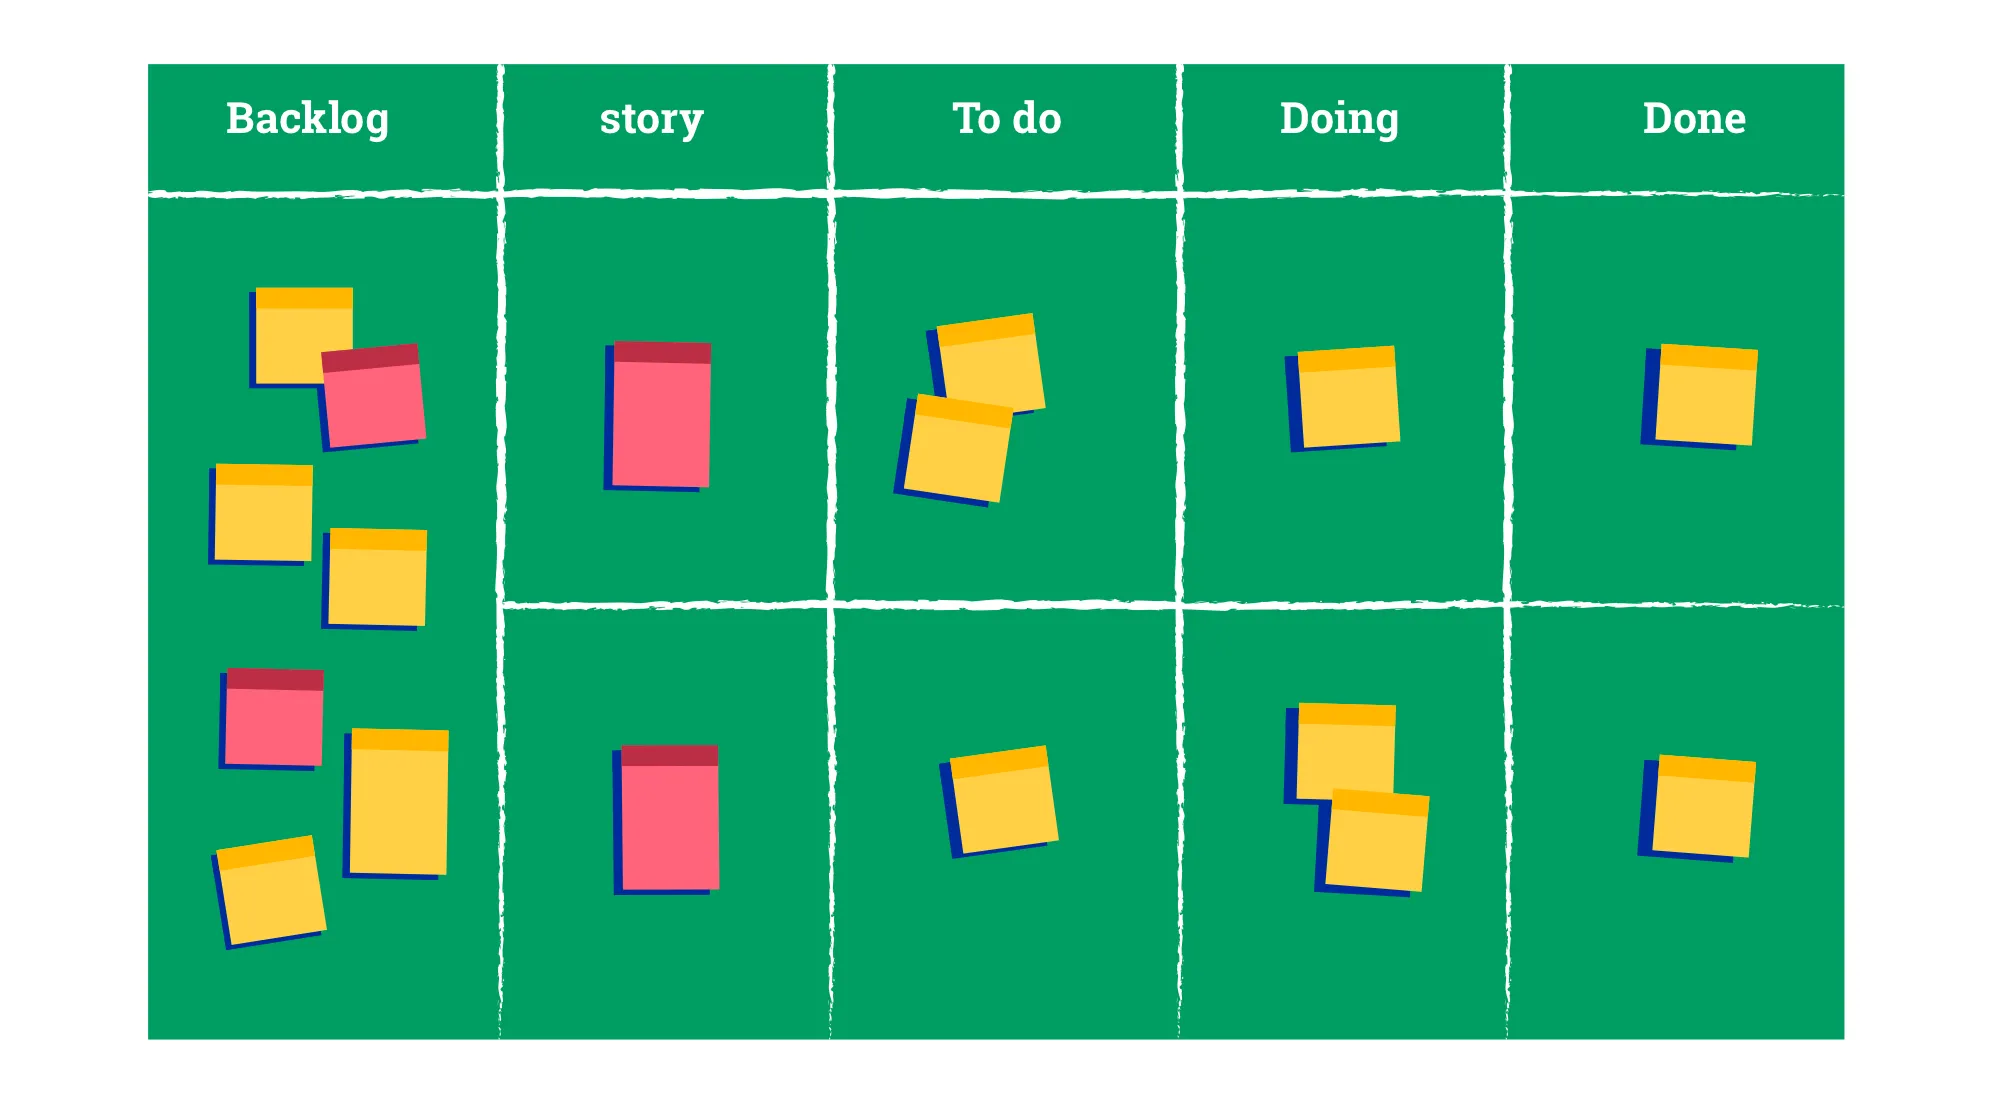
\includegraphics[width=0.8\columnwidth]{capitolo1/scrumb-board.png}
  \caption{Esempio di organizzazione delle attività nella Scrum Board}
\end{figure}

Un altro evento fondamentale che fa parte di Scrum, al quale ho avuto modo di partecipare, è lo \textbf{\textit{sprint review}}. Quest'ultimo consiste in una riunione di fine sprint in cui si ispezionano i risultati dell'incremento insieme agli \textit{stakeholders}, decidendo eventuali cambiamenti da apportare al \textit{product backlog}. \\

\subsection{Manutenzione}
In seguito al rilascio di un \textit{software}, l'azienda si impegna a seguire la sua naturale evoluzione nel tempo, adattandolo sempre a nuove esigenze, e a risolvere eventuali errori. Per questo Sync Lab offre servizi di manutenzione che possono essere di tre tipi:
\begin{itemize}
  \item \textbf{Manutenzione correttiva}: permette di correggere eventuali difetti del prodotto;
  \item \textbf{Manutenzione adattiva}: permette di adattare il \textit{software} a cambiamenti dell'ambiente operativo;
  \item \textbf{Manutenzione evolutiva}: permette di estendere le funzionalità del prodotto esistente.
\end{itemize}

\section{Tecnologie utilizzate}
Da quel che ho potuto constatare durante l'attività di stage, per la realizzazione dei prodotti sopra elencati Sync Lab sfrutta un'ampia gamma di tecnologie per fornire prodotti stabili e sicuri. Le tecnologie utilizzate sono molte e variano in base alla necessità del prodotto, ma quelle più utilizzate possono essere raggruppate in due grandi categorie: \textit{front-end} e \textit{back-end}. \\

Per quanto riguarda le tecnologie di supporto, c'è stato un aumento di utilizzo dei sistemi di comunicazione digitali a causa della pandemia, anche se venivano già utilizzati precedentemente per comunicare con le diverse sedi. La pandemia ha spinto Sync Lab ad un utilizzo sempre maggiore di Discord, Google Meet, Trello e Notion.

\begin{itemize}
  \item \textbf{Google Meet}: \textit{software} utilizzato per le videoconferenze che permette di comunicare con più colleghi aziendali e organizzare riunioni virtuali con un grande numero di partecipanti;
  \item \textbf{Discord}: piattaforma di comunicazione digitale gratuita, la quale permette di fruire di chat in tempo reale, gestendo più canali vocali e testuali divisi per argomento. Tra le varie funzioni disponibili, permette di dividere i membri in gruppi in base al progetto che devono portare a termine. È presente anche una sezione per le videoconferenze, ma è meno avanzata rispetto a Google Meet e per questo non lo si preferisce;
  \item \textbf{Trello}: piattaforma per la gestione di progetti seguendo la metodologia Scrum. Trello mette a disposizione una \textit{Scrum Board} dove è possibile dividere le attività in base al loro stato di avanzamento. Le colonne sono modificabili, come qualsiasi componente in Trello, ma quelle predefinite sono le seguenti:
  \begin{itemize}
    \item \textbf{Backlog}: contiene il \textit{product backlog};
    \item \textbf{Da fare}: definisce le attività da svolgere durante lo \textit{sprint};
    \item \textbf{In corso}: presenta tutte le attività in esecuzione;
    \item \textbf{In verifica}: consiste in tutte le attività in attesa di verifica;
    \item \textbf{Terminati}: include le attività legate ad uno \textit{sprint} che sono state verificate. 
  \end{itemize}
  \item \textbf{Notion}: piattaforma utilizzata per la prenotazione del posto in sede, così da facilitare la gestione ed il controllo delle persone, in modo tale da rispettare il numero massimo consentito dalla legge.
\end{itemize}

\subsection{Front-end}
Le tecnologie per lo sviluppo di interfacce grafiche utilizzate da Sync Lab sono le seguenti:

\paragraph{Linguaggi di programmazione} 
I linguaggi di programmazione più utilizzati sono \textbf{Javascript}, impiegato nella realizzazione di applicativi web interattivi, \textbf{kotlin}, un linguaggio multi-paradigma che sta sempre più prendendo piede per lo sviluppo di applicazioni android, e \textbf{Swift}, per lo sviluppo di applicazioni IOS. Sempre di più si sta puntando su \textbf{Typescript}, un \textit{superset} di Javascript, al quale aggiunge tipi, classi e interfacce.

\paragraph{Framework}
L'ambito web è quello dove avviene un impiego maggiore di \textit{framework}. I più utilizzati sono attualmente due: Angular e React.js. \textbf{Angular} è uno dei \textit{framework} open-source più popolari e utilizzati al mondo per lo sviluppo di \gls{Single Page Application}. Permette di creare applicazioni web di livello \textit{enterprise} grazie a una serie di funzionalità e strumenti, utilizzando come linguaggio principale Typescript. \textbf{React.js}, invece, si distingue da Angular per la maggiore facilità di apprendimento e velocità a livello di \textit{performance}, la quale lo rende perfetto per la realizzazione di siti semplici. Un altro \textit{framework} che sta sempre di più prendendo piede all'interno dell'azienda, anche se di fatto non è ancora stato adottato ufficialmente, è \textbf{Vue.js}. Molto simile a React.js, Vue.js introduce il concetto di \gls{Single File Components}, semplificando maggiormente la scrittura di applicazioni web.

\subsection{Back-end}
Per quanto riguarda le tecnologie per lo sviluppo lato \textit{back-end}, si possono identificare le seguenti:

\paragraph{Linguaggi di programmazione}
\textbf{Java} e \textbf{Scala}, due linguaggi basati sulla \textit{Java Virtual Machine}, fanno da padrone per lo sviluppo lato \textit{back-end}. Entrambi sono linguaggi maturi ed ampiamente utilizzati in questo mondo, con una grande varietà di librerie e \textit{framework}. Vengono sfruttati principalmente per lo sviluppo di servizi \textit{REST} in ambito web.

\paragraph{Framework}
Il \textit{framework} più utilizzato per lo sviluppo in questo ambito è sicuramente \textbf{Spring}. Quest'ultimo permette di realizzare applicativi lato \textit{server} utilizzando il linguaggio Java e sfruttando vari \textit{design patterns}. La scelta dell'architettura è totalmente libera e Spring si presta perfettamente a qualunque tipologia si voglia scegliere.

\section{Propensione all'innovazione}
Sync Lab è un'azienda in costante aggiornamento che guarda all'innovazione con grande interesse, per garantire soluzioni software sempre rivoluzionarie. Simbolo di questo sforzo da parte dell'azienda è anche la grande quantità di collaborazioni con le principali università d'Italia (università degli studi di Padova, politecnico di Milano, università degli studi Federico II, ecc.) e vari enti europei.\\

\begin{figure}[!h]
  \centering
  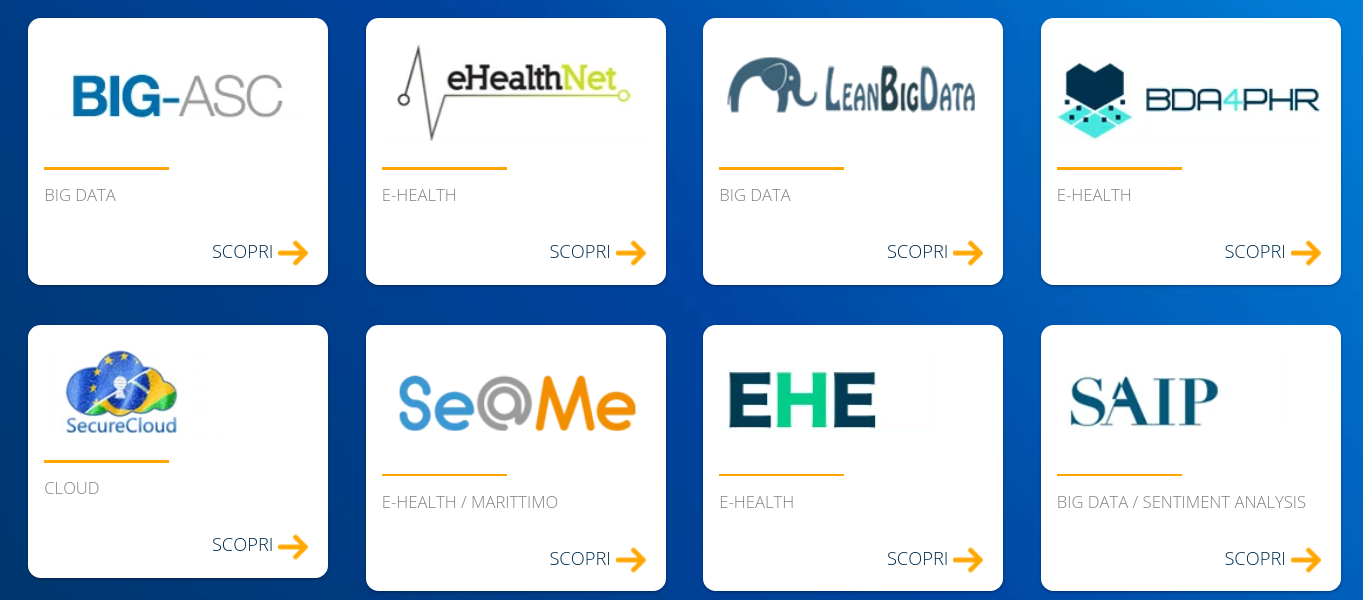
\includegraphics[width=\textwidth]{capitolo1/prodotti-ricerca-sviluppo.png}
  \caption{Alcuni progetti di ricerca e sviluppo di Sync Lab}
  \textbf{Fonte}: \href{https://www.synclab.it/ricerca-e-sviluppo.php}{https://www.synclab.it/ricerca-e-sviluppo.php}
\end{figure}

Per adempiere al meglio al difficile compito di restare sempre aggiornati sulle ultime tecnologie, Sync Lab è divisa in tre dipartimenti:
\begin{itemize}
  \item \textbf{\textit{Research and Development (R\&D)}}: dove l'azienda promuove nuovi prodotti eseguendo ricerca e sviluppo in più settori, alimentando così il profilo aziendale e le proprie competenze nel mercato;
  \item \textbf{\textit{Lab}}: in cui l'azienda mette in atto i risultati derivanti dal dipartimento \textit{R\&D}, promuovendo soluzioni che migliorino ed estendano l'innovazione tecnologica;
  \item \textbf{\textit{Start-up}}: dove l'azienda collabora e promuove le \textit{start-up} con maggiore successo in termini di innovazione, sia in Italia che all'estero.
\end{itemize}  

L'azienda, inoltre, sta approfondendo sempre di più gli ambiti di \textit{Cybersecurity}, \textit{E-Health}, \textit{Blockchain} e \textit{Big Data}, formando degli appositi progetti di ricerca nelle diverse sedi per sperimentare e imparare nuove tecnologie. \\

Un evento che ho trovato interessante e mi è piaciuto molto durante il mio tirocinio, è stato il "Paola presenta". 
Questa ricorrenza, che in genere è settimanale, consiste in un'ora di presentazione su un argomento proposto da un dipendente. L'argomento della presentazione può riguardare qualcosa sulla quale sta lavorando, oppure semplicemente si è interessato. 
Ogni dipendente è libero di partecipare e, su richiesta, può presentare lui stesso un argomento a piacere. Questo evento l'ho trovato molto interessante e dimostra quanto i colleghi di Sync Lab vogliano sempre stare aggiornati ed informati su tutto quello che interessa il mondo informatico. 
Personalmente ho partecipato a tre di queste presentazioni: una dove hanno introdotto la tecnologia \textit{Blockchain}, tenuta dal mio \textit{tutor} aziendale Fabio Pallaro, un'altra dove hanno spiegato come funzionano gli strumenti che compongono la \textit{Elastick Stack} e l'ultima dove hanno parlato dell'analisi statica del codice con la piattaforma \textit{SonarQube}. \\

Questa propensione all'innovazione l'ho avvertita anche nel mio progetto di stage, dove non ho trattato tecnologie usuali, ma ho dovuto studiare e approfondire tecnologie che attualmente non sono così diffuse in ambito \textit{enterprise}, ma sicuramente rappresentano un'importante \textit{milestone} nella storia dell'informatica.
             % Capitolo 1
% !TEX encoding = UTF-8
% !TEX TS-program = pdflatex
% !TEX root = ../tesi.tex

\chapter{Lo stage}
\label{cap:stage}

\section{Scelta dell'azienda}
Ragione per la quale ho scelto il seguente stage a discapito di altri, approfondendo la motivazione per la quale l'azienda ha scelto di intraprendere questo percorso.

\section{Il progetto}
Spiegazione approfondita del progetto di stage, con una breve introduzione al contesto sul quale si basa.

\section{Obiettivi dello stage}
Approfondimento degli obiettivi e prodotti attesi del mio stage.

\section{Obiettivi personali}
Descrizione degli obiettivi definiti nel piano di lavoro.

\section{Vincoli dello stage}

\subsection{Pianificazione temporale}
Presentazione della pianificazione temporale.

\subsection{Vincoli organizzativi}
Spiegazione delle modalità di lavoro intraprese sia con il tutor aziendale, sia con il mio relatore, approfondendo gli strumenti utilizzati.

\section{Analisi dei rischi}
Breve analisi dei rischi.
             % Processi
% !TEX encoding = UTF-8
% !TEX TS-program = pdflatex
% !TEX root = ../tesi.tex

\chapter{Il progetto: NFTLab}
\label{cap:nftlab}

%%%%%%%%%%%%%%%%%%%%%%%%%%%%%%%%%%%%%%%%%%%%%%%%%%%%%%%%%%%%%%%%%%%%%%%%%%%%%%%%%

\section{Analisi dei rischi}
Breve analisi dei rischi.

\section{Studio preliminare}

\subsection{Cos'è la blockchain}
Spiegazione di cos'è la blockchain, introducendo la blockchain di BitCoin come termine di paragone per quelle interessate nel mio stage.

\subsubsection{Il \textit{wallet}}
Cos'è il wallet, come viene creato, gestito e il ruolo che ha durante le transazioni nella blockchain.

\subsubsection{Il ruolo importante dei \textit{miners}}
Chi sono i miners e il concetto di rewards in base al processo che svolgono, approfondendo i vari tipi di proof-of-X.

\subsubsection{La crittografia in gioco}
Spiegazione dei sistemi crittografici in gioco nella blockchain.

\subsubsection{Composizione di un blocco in BitCoin}
Com'è composto un blocco in BitCoin.

\subsubsection{Come si svolge una transazione e la sua composizione}
Processo intrapreso da una transazione in BitCoin e la sua composizione.

\subsubsection{Le diramazioni in BitCoin}
Essendo la blockchain un sistema distribuito, qui verrà spiegato come bitcoin gestisce le diramazioni che si generano casualmente.

\subsubsection{I possibili attacchi alla blockchain}
Breve introduzione alla sicurezza della blockchain e dei possibili attacchi a cui può essere sottoposta.

\subsection{La blockchain Ethereum}
Introduzione alla blockchain Ethereum spiegando le differenze con BitCoin.

\subsubsection{Il concetto di smart contract}
Cos'è uno smart contract, introduzione al concetto di gas limit e gas price e il linguaggio Solidity.

\subsubsection{Tipi di transazioni}
Approfondimento dei vari tipi di transazioni che si possono compiere in Ethereum.

\subsubsection{Lo stato di Ethereum}
Come viene gestito lo stato di Ethereum e spiegazione della struttura dati merkle patricia tries.

\subsubsection{Composizione di un blocco}
Com'è composto un blocco in Ethereum e differenze rispetto a BitCoin.

% \paragraph{\textit{Merkle Patricia tries}}

\subsection{La blockchain Hotmoka}
Introduzione alla blockchain Hotmoka spiegando le differenze con Ethereum.

\subsubsection{Cos'è Tendermint e il suo utilizzo in Hotmoka}
Spiegazione di cos'è Tendermint e di come viene utilizzato in Hotmoka.

\subsubsection{Lo stato di Hotmoka}
Come viene gestito lo stato in Hotmoka.

\subsubsection{Gli smart contract in Hotmoka}
Come vengono gestiti gli smart contract in Hotmoka e il linguaggio Takamaka.

\subsection{Lo standard ERC721}
Cos'è lo standard ERC721 per la gestione di NFT.

\subsection{Il protocollo IPFS (InterPlanetary File System)}
Cos'è il protocollo IPFS e come si può utilizzare per la gestione di NFT.

%%%%%%%%%%%%%%%%%%%%%%%%%%%%%%%%%%%%%%%%%%%%%%%%%%%%%%%%%%%%%%%%%%%%%%%%%%%%%%%%%

\section{Strumenti e configurazione}

\subsection{Strumenti di gestione del progetto}
Descrizione degli strumenti utilizzati per la gestione del progetto.

\subsection{Documentazione}
Descrizione degli strumenti utilizzati per la scrittura della documentazione e dei vari diagrammi UML.

\subsection{Ambiente di sviluppo}
Descrizione dell'ambiente di sviluppo utilizzato.

\subsection{Tecnologie usate}
Descrizione dei vari linguaggi di programmazione, framework, librerie e strumenti di build automation.

\subsection{Analisi statica del codice}
Descrizione degli strumenti utilizzati per l'automazione dell'analisi statica del codice.

\subsection{Way of working}
Spiegazione di come viene organizzato e gestito il flusso di sviluppo.

%%%%%%%%%%%%%%%%%%%%%%%%%%%%%%%%%%%%%%%%%%%%%%%%%%%%%%%%%%%%%%%%%%%%%%%%%%%%%%%%%

\section{Analisi dei requisiti}

\subsection{Casi d'uso}

\subsubsection{Attori primari}
Elenco e spiegazione degli attori primari.

\subsubsection{Attori secondari}
Elenco e spiegazione degli attori secondari.

\subsubsection{Diagrammi dei casi d'uso}
Tutti i vari diagrammi dei casi d'uso.

% \paragraph{UC1 - Caricamento di un opera in blockchain}

% \paragraph{UC2 - Vendita di un opera}

% \paragraph{UC3 - Ottenimento di un opera a partire dal suo id}

% \paragraph{UC4 - Ottenimento di un opera a partire dal suo hash}

\subsection{Requisiti funzionali}
Tabella dei requisiti funzionali, con relativa spiegazione e fonte.

\subsection{Requisiti di qualità}
Tabella dei requisiti di qualità, con relativa spiegazione e fonte.

\subsection{Requisiti di vincolo}
Tabella dei requisiti di vincolo, con relativa spiegazione e fonte.

%%%%%%%%%%%%%%%%%%%%%%%%%%%%%%%%%%%%%%%%%%%%%%%%%%%%%%%%%%%%%%%%%%%%%%%%%%%%%%%%%

\section{Smart contract per Ethereum}
Spiegazione dello scopo e dei compiti dello smart contract per Ethereum.

\subsection{Progettazione}
Scelte progettuali, best practices impiegate e design pattern che sono stati utilizzati. 

\subsubsection{Architettura}
Presentazione dell'architettura con diagrammi di package, classe e sequenza.

\subsection{Codifica}
Spiegazione di quanto fatto durante il periodo di codifica, approfondendo parti di codice che ritengo importanti.

\subsection{Verifica}
Spiegazione delle librerie attraverso le quali sono stati implementati i test, numero di test scritti e code coverage raggiunto.

%%%%%%%%%%%%%%%%%%%%%%%%%%%%%%%%%%%%%%%%%%%%%%%%%%%%%%%%%%%%%%%%%%%%%%%%%%%%%%%%%

\section{Lo standard ERC721 per Hotmoka}
Spiegazione del perché è risultata necessaria la scrittura dello standard ERC721 per Hotmoka.

\subsection{Progettazione}
Scelte progettuali, best practices impiegate e design pattern che sono stati utilizzati. 

\subsubsection{Architettura}
Presentazione dell'architettura con diagrammi di package, classe e sequenza.

\subsection{Codifica}
Spiegazione di quanto fatto durante il periodo di codifica, approfondendo parti di codice che ritengo importanti.

\subsection{Verifica}
Spiegazione delle librerie attraverso le quali sono stati implementati i test, numero di test scritti e code coverage raggiunto.

%%%%%%%%%%%%%%%%%%%%%%%%%%%%%%%%%%%%%%%%%%%%%%%%%%%%%%%%%%%%%%%%%%%%%%%%%%%%%%%%%

\section{Smart contract per Hotmoka}
Spiegazione dello scopo e dei compiti dello smart contract per Hotmoka.

\subsection{Progettazione}
Scelte progettuali, best practices impiegate e design pattern che sono stati utilizzati. 

\subsubsection{Architettura}
Presentazione dell'architettura con diagrammi di package, classe e sequenza.

\subsection{Codifica}
Spiegazione di quanto fatto durante il periodo di codifica, approfondendo parti di codice che ritengo importanti.

\subsection{Verifica}
Spiegazione delle librerie attraverso le quali sono stati implementati i test, numero di test scritti e code coverage raggiunto.

%%%%%%%%%%%%%%%%%%%%%%%%%%%%%%%%%%%%%%%%%%%%%%%%%%%%%%%%%%%%%%%%%%%%%%%%%%%%%%%%%

\section{Libreria per l'integrazione con gli smart contract}
Spiegazione dello scopo e dei compiti della libreria per l'integrazione con gli smart contract.

\subsection{Progettazione}
Scelte progettuali, best practices impiegate e design pattern che sono stati utilizzati. 

\subsubsection{Architettura}
Presentazione dell'architettura con diagrammi di package, classe e sequenza.

\subsection{Codifica}
Spiegazione di quanto fatto durante il periodo di codifica, approfondendo parti di codice che ritengo importanti.

\subsection{Verifica}
Spiegazione delle librerie attraverso le quali sono stati implementati i test, numero di test scritti e code coverage raggiunto.

%%%%%%%%%%%%%%%%%%%%%%%%%%%%%%%%%%%%%%%%%%%%%%%%%%%%%%%%%%%%%%%%%%%%%%%%%%%%%%%%%

\section{Validazione e collaudo}
Riassunto dei requisiti soddisfatti e risultato del collaudo.

%%%%%%%%%%%%%%%%%%%%%%%%%%%%%%%%%%%%%%%%%%%%%%%%%%%%%%%%%%%%%%%%%%%%%%%%%%%%%%%%%

\section{Resoconto dei prodotti sviluppati}
Quantità di prodotti software che sono stati sviluppati (in termini di linee di codice) e numero di documenti prodotti.

%%%%%%%%%%%%%%%%%%%%%%%%%%%%%%%%%%%%%%%%%%%%%%%%%%%%%%%%%%%%%%%%%%%%%%%%%%%%%%%%%

\section{Integrazione del prodotto in NFTLab}
Come quanto è stato implementato si integra all'interno del prodotto NFTLab.

%%%%%%%%%%%%%%%%%%%%%%%%%%%%%%%%%%%%%%%%%%%%%%%%%%%%%%%%%%%%%%%%%%%%%%%%%%%%%%%%%

\section{Le conclusioni}
Considerazioni conclusive sul confronto tra le due blockchain Hotmoka e Ethereum.
             % Kick-Off
% !TEX encoding = UTF-8
% !TEX TS-program = pdflatex
% !TEX root = ../tesi.tex

%**************************************************************
\chapter{Valutazione finale}
\label{cap:valutazione-finale}
%**************************************************************

\section{Raggiungimento degli obiettivi}
Resoconto del completamento degli obiettivi di stage e di prodotto.

% \subsection{Obiettivi di stage}

% \subsection{Obiettivi di prodotto}

\section{Competenze e conoscenze maturate}
Quanto ho appreso e quali conoscenze ho maturato in seguito a questo stage.

\section{Differenza tra il mondo universitario e il lavoro}
Descrizione della distanza che ho trovato tra le competenze richieste a inizio stage e quelle erogate dal corso di studi.
             % Concept Preview
% \input{capitoli/capitolo-5}             % Product Prototype
% \input{capitoli/capitolo-6}             % Product Design Freeze e SOP
% \input{capitoli/capitolo-7}             % Conclusioni
\appendix                               
% % !TEX encoding = UTF-8
% !TEX TS-program = pdflatex
% !TEX root = ../tesi.tex

%**************************************************************
\chapter{Appendice A}
%**************************************************************

\epigraph{Citazione}{Autore della citazione}             % Appendice A

%**************************************************************
% Materiale finale
%**************************************************************
\backmatter
\printglossary[title={Glossario}]
\printglossary[type=\acronymtype, title={Acronimi}]
% !TEX encoding = UTF-8
% !TEX TS-program = pdflatex
% !TEX root = ../tesi.tex

%**************************************************************
% Bibliografia
%**************************************************************

\cleardoublepage
\chapter{Bibliografia e Sitografia}
\label{cap:bibliografia-sitografia}

\nocite{*}
% Stampa i riferimenti bibliografici
\printbibliography[heading=subbibliography,title={Riferimenti bibliografici},type=book]

% Stampa i siti web consultati
\printbibliography[heading=subbibliography,title={Siti web consultati},type=online]


\end{document}
